% This is "sig-alternate.tex" V2.0 May 2012
% This file should be compiled with V2.5 of "sig-alternate.cls" May 2012
%
% This example file demonstrates the use of the 'sig-alternate.cls'
% V2.5 LaTeX2e document class file. It is for those submitting
% articles to ACM Conference Proceedings WHO DO NOT WISH TO
% STRICTLY ADHERE TO THE SIGS (PUBS-BOARD-ENDORSED) STYLE.
% The 'sig-alternate.cls' file will produce a similar-looking,
% albeit, 'tighter' paper resulting in, invariably, fewer pages.
%
% ----------------------------------------------------------------------------------------------------------------
% This .tex file (and associated .cls V2.5) produces:
%       1) The Permission Statement
%       2) The Conference (location) Info information
%       3) The Copyright Line with ACM data
%       4) NO page numbers
%
% as against the acm_proc_article-sp.cls file which
% DOES NOT produce 1) thru' 3) above.
%
% Using 'sig-alternate.cls' you have control, however, from within
% the source .tex file, over both the CopyrightYear
% (defaulted to 200X) and the ACM Copyright Data
% (defaulted to X-XXXXX-XX-X/XX/XX).
% e.g.
% \CopyrightYear{2007} will cause 2007 to appear in the copyright line.
% \crdata{0-12345-67-8/90/12} will cause 0-12345-67-8/90/12 to appear in the copyright line.
%
% ---------------------------------------------------------------------------------------------------------------
% This .tex source is an example which *does* use
% the .bib file (from which the .bbl file % is produced).
% REMEMBER HOWEVER: After having produced the .bbl file,
% and prior to final submission, you *NEED* to 'insert'
% your .bbl file into your source .tex file so as to provide
% ONE 'self-contained' source file.
%
% ================= IF YOU HAVE QUESTIONS =======================
% Questions regarding the SIGS styles, SIGS policies and
% procedures, Conferences etc. should be sent to
% Adrienne Griscti (griscti@acm.org)
%
% Technical questions _only_ to
% Gerald Murray (murray@hq.acm.org)
% ===============================================================
%
% For tracking purposes - this is V2.0 - May 2012

\documentclass{sig-alternate}
\usepackage{fixltx2e}
\usepackage{xcolor}
\def\SPSB#1#2{\rlap{\textsuperscript{\textcolor{red}{#1}}}\SB{#2}}
\def\SP#1{\textsuperscript{\textcolor{black}{#1}}}
\def\SB#1{\textsubscript{\textcolor{black}{#1}}}
\newenvironment{myquote}
               {\list{}{\rightmargin   \leftmargin
                        \parsep        0in }%
                \item\relax}
               {\endlist}
\newcommand{\userquote}[2]{\begin{samepage}\begin{myquote} 
     \em{\small{#2\begin{flushright}---#1\end{flushright}}}
   \end{myquote}\end{samepage}}
%Quote code
%\newif\ifquoteopen
%\catcode`\"=\active % lets you define `"` as a macro
%\DeclareRobustCommand*{"}{%
%   \ifquoteopen
%     \quoteopenfalse ''%
%   \else
%     \quoteopentrue ``%
%   \fi
%}

%End of quote code

\begin{document}
%
% --- Author Metadata here ---
\conferenceinfo{ICTD'16,}{June 3-6, 2016, Ann Arbor, Michigan, USA}
%\CopyrightYear{2007} % Allows default copyright year (20XX) to be over-ridden - IF NEED BE.
%\crdata{0-12345-67-8/90/01}  % Allows default copyright data (0-89791-88-6/97/05) to be over-ridden - IF NEED BE.
% --- End of Author Metadata ---

%\title{Alternate {\ttlit ACM} SIG Proceedings Paper in LaTeX
%\title{Leveraging on Families' Social Interactions on Utilization of Personal Health Informatics through Intermediaries}
\title{Leveraging Intermediated Interactions to Support Utilization of Persuasive Personal Health Informatics}
%
% You need the command \numberofauthors to handle the 'placement
% and alignment' of the authors beneath the title.
%
% For aesthetic reasons, we recommend 'three authors at a time'
% i.e. three 'name/affiliation blocks' be placed beneath the title.
%
% NOTE: You are NOT restricted in how many 'rows' of
% "name/affiliations" may appear. We just ask that you restrict
% the number of 'columns' to three.
%
% Because of the available 'opening page real-estate'
% we ask you to refrain from putting more than six authors
% (two rows with three columns) beneath the article title.
% More than six makes the first-page appear very cluttered indeed.
%
% Use the \alignauthor commands to handle the names
% and affiliations for an 'aesthetic maximum' of six authors.
% Add names, affiliations, addresses for
% the seventh etc. author(s) as the argument for the
% \additionalauthors command.
% These 'additional authors' will be output/set for you
% without further effort on your part as the last section in
% the body of your article BEFORE References or any Appendices.

\numberofauthors{3} %  in this sample file, there are a *total*
% of EIGHT authors. SIX appear on the 'first-page' (for formatting
% reasons) and the remaining two appear in the \additionalauthors section.
%
\author{
% You can go ahead and credit any number of authors here,
% e.g. one 'row of three' or two rows (consisting of one row of three
% and a second row of one, two or three).
%
% The command \alignauthor (no curly braces needed) should
% precede each author name, affiliation/snail-mail address and
% e-mail address. Additionally, tag each line of
% affiliation/address with \affaddr, and tag the
% e-mail address with \email.
%
% 1st. author
\alignauthor
        Ntwa Katule \\
        %\affaddr{Institute for Clarity in Documentation}\\
        %\affaddr{1932 Wallamaloo Lane}\\
       % \affaddr{Wallamaloo, New Zealand}\\
        %\email{trovato@corporation.com}
% 2nd. author
\alignauthor
Melissa Densmore\\
        %\affaddr{Institute for Clarity in Documentation}\\
        %\affaddr{P.O. Box 1212}\\
        %\affaddr{Dublin, Ohio 43017-6221}\\
       % \email{webmaster@marysville-ohio.com}
% 3rd. author
\alignauthor Ulrike Rivett\\
       %\affaddr{The Th{\o}rv{\"a}ld Group}\\
        %\affaddr{1 Th{\o}rv{\"a}ld Circle}\\
        %\affaddr{Hekla, Iceland}\\
        %\email{larst@affiliation.org}
%\and  % use '\and' if you need 'another row' of author names
% 4th. author
%\alignauthor Lawrence P. Leipuner\\
%       \affaddr{Brookhaven Laboratories}\\
%       \affaddr{Brookhaven National Lab}\\
%       \affaddr{P.O. Box 5000}\\
%       \email{lleipuner@researchlabs.org}
% 5th. author
%\alignauthor Sean Fogarty\\
%       \affaddr{NASA Ames Research Center}\\
%       \affaddr{Moffett Field}\\
%       \affaddr{California 94035}\\
%       \email{fogartys@amesres.org}
% 6th. author
%\alignauthor Charles Palmer\\
%       \affaddr{Palmer Research Laboratories}\\
%       \affaddr{8600 Datapoint Drive}\\
%       \affaddr{San Antonio, Texas 78229}\\
%       \email{cpalmer@prl.com}
}
% There's nothing stopping you putting the seventh, eighth, etc.
% author on the opening page (as the 'third row') but we ask,
% for aesthetic reasons that you place these 'additional authors'
% in the \additional authors block, viz.
%\additionalauthors{Additional authors: John Smith (The Th{\o}rv{\"a}ld Group,
%email: {\texttt{jsmith@affiliation.org}}) and Julius P.~Kumquat
%(The Kumquat Consortium, email: {\texttt{jpkumquat@consortium.net}}).}
\date{30 July 1999}
% Just remember to make sure that the TOTAL number of authors
% is the number that will appear on the first page PLUS the
% number that will appear in the \additionalauthors section.

\maketitle 

\begin{abstract} 
Behavior change support systems (BCSS) and
persuasive technologies for healthcare often entail users interacting with
mobile devices. However, especially in developing countries, the target
community is unfamiliar with and often intimidated by new technologies.  In
this paper we propose the use of  {\em{intermediaries}} to facilitate
interaction with a mobile phone-based application and to motivate ongoing use
by the target beneficiaries. The application incentivizes utilization through
gamification techniques, using badges, scoreboards, and other rewards.  For
example, a young girl might help her father keep track of his walking and
diet, maintaining participation as much for her father's health as for the
social awards given by the app.  We explain how intermediaries can be
leveraged to improve utilization and engagement of the beneficiaries, and
describe factors affecting interaction between the participating pairs and
interaction with the application. This study highlights the importance of
social rapport - typically through a familial relationship - as a key
component of the intervention. Finally, we discuss the implications of
designing for the motivation of two different users: gamification,
personalization and utility play different roles for the intermediary and the
beneficiary but ultimately combine to make a more effective application for
the beneficiary than one targeting the beneficiary alone. 
\end{abstract}

% A category with the (minimum) three required fields
\category{H.5m.}{Information interfaces and presentation}{Miscellaneous}
\category{H.1.2.}{User/Machine Systems}{Human Factors}
%A category including the fourth, optional field follows...
\keywords{HCI4D, intermediated interactions, persuasive technologies, gamification, personal informatics, motivational affordances, health}

\section{Introduction} Approximately 1.3 billion people are considered to be
either overweight or obese worldwide, of which two-thirds are found in low-
income or developing countries ~\cite{Steyn2006}. While this pandemic used to
be considered a ``first world problem'', urbanization and changing lifestyles
have led to increasing problems for the low-income communities of the
developing world. For example, 60\% of South Africans are overweight, with
four in 10 women that are either overweight or clinically
obese~\cite{ng:global}.

A typical intervention from the West might entail development of a persuasive
application to encourage healthy eating and exercise behaviors
~\cite{arsand:mobile,hamari2014persuasive}.  Persuasive applications on mobile
phones are particularly well-positioned for interventions that target
psychological processes, because they are pervasively present for the users
~\cite{hsu2014persuasive}. Gamification, enabling self-reflection, or more
simple strategies such as SMS-based reminders all motivate positive
experiences and more frequent engagement
~\cite{hamari2014persuasive,cole2010text} The subset of these interventions
that target collection of personal history entry, review and analysis is
broadly called personal informatics, or personal health informatics (PHI) for
health interventions.

However these applications fail to replicate well to typical populations
targeted by information and communications technology for development (ICTD)
interventions ~\cite{kaplan2006can}. In part this is due to problems of
technology access: people do not own phones, share phones, or do not know how
to use them.  In the context of obesity, many potential target users are
older, further exacerbating the problem. As a result, more typical ICTD
interventions target community health workers (CHWs) or other intermediaries
as facilitators of access to mobile content
~\cite{ramachandran2010mobile,ramachandran2010research,molapo2013software}.
However, Sambasivan et al suggest another resource - young girls and boys in
the community can be leveraged as intermediaries for older adults seeking to
interact with new technologies ~\cite{sambasivan2010}. Thus, we propose that
persuasive PHI might be more effective if it incorporates intermediaries to
motivate participation.

In this paper, we present the results of a series of studies conducted in two
townships in Cape Town, South Africa. In these studies, we have deployed a
mobile application to support PHI for overweight or pre-diabetic adults. The
application primarily incorporates gamification strategies such as challenges,
badges, and leaderboards for motivating ongoing use. Each adult elects an
intermediary to assist with use of the application, and is given airtime to
use the application for two to six weeks. We identify characteristics of
effective intermediaries, highlighting social rapport as a key contributor
towards effectiveness of the application. Using qualitative feedback from
participants, we also discuss important aspects of intermediated interaction
and implications of intermediation on design of persuasive technologies.
Ultimately we find that intermediated persuasive technologies are an effective
way to improve engagement of adults with PHI.

\section{Related Work} 

Persuasive technologies have evolved from prescriptive
nature of information flow in between health care providers and health care
recipients ~\cite{chatterjee2009healthy} to behaviour change support systems
(BCSS) ~\cite{langrial2012digital}. Oinas-kukkonen 
~\cite{Oinas-Kukkonen:foundation} defined BCSS as ``a socio-technical information system
with psychological and behavioural outcomes designed to form, alter or
reinforce attitudes, behaviours or an act of complying without using coercion
or deception''.

In order for a system to be persuasive, the persuasion goal in design must be
intentional ~\cite{hamari2014persuasive}. The persuasive system design (PSD) model
proposes a set of functionalities required for a system to be considered a
persuasive technology ~\cite{Oinas-kukkonen:psd}. The first set of
functionalities fall under primary task support, which includes but is not limited
to: reduction of complex behaviours into simple tasks; guiding the user
through experiences while persuade along the way; tailoring of persuasive
information to factors relevant to a user group; personalization of content;
and self-monitoring for users to keep track of their performance in  achieving
goals. The second set of functionalities fall under dialogue support, which includes
praises, rewards, reminders, similarity, liking, and social roles. The third
set functionalities fall under system credibility support, which includes
trustworthiness, expertise, surface credibility etc. The last set of
functionalities emphasize the role of social support, which includes social
learning, social comparison, and competition.

Gamification is also garnering popularity as a means to
persuade people because of its ability to invoke users' intrinsic experiences
through gameful experiences ~\cite{hamari2014persuasive}. Gamification is the
use of game design elements in non-game contexts ~\cite{deterding2011game} with
an objective of increasing engagement in a particular activity. A systematic
review on peer reviewed studies found that gamification provides positive
effects and these effects are highly dependent on both the context in which
gamification is implemented and the users using it ~\cite{hamari2014does}.
Hamari and Koivisto ~\cite{hamari2013social} found out that social motivations
for use of a gamified service/system are attributed to social influence,
recognition, reciprocal benefit, and network exposure. Some of these
attributes resonate with the functionality proposed on the aforementioned PSD
model for BCSS.

Typically a BCSS will aim at sustaining engagement over a long period of time
~\cite{Oinas-Kukkonen:foundation}, but only considers single users. 
Existing literature does not consider how to design systems that include 
intermediaries
as part of the engagement. In this work, we seek to understand how
can one sustain engagement in the context of intermediated interactions. We
explore important human factors in intermediated interactions that may affect
utilization of persuasive personal health informatics (PHI) that target health
behavior change. In the next sub-sections, we discuss literature on social
relationships in the context of intermediated technology use, and utilization
of human intermediaries in health behavior change through ICTs.

\subsection{Intermediaries in ICTs for Healthy Behavior Change}

In the context of ICTD, human intermediaries have been previously utilized on
behavior change interventions. One study
~\cite{ramachandran2010mobile,ramachandran2010research} in India used community
health workers (CHWs) with help of mobile messages to persuade pregnant and postnatal
women together with their relatives on maternal health issues.  Community
health workers interacted with mobile phones to access persuasive messages to
share with their clients. Another study by Molapo and Marsden
~\cite{molapo2013software}  empowered rural health trainers with a software
application that allows them to create digital  training  content  for 
low-literate 
CHWs in Lesotho, using images, voice-over, and  video clips.
While intended only for training, CHWs also chose to save those videos with their 
clients, having the unintentional
effect of persuading people to get tested for diseases such as
tuberculosis. In this context CHWs were acting as intermediaries as they
provided access to information that had persuasive effects. 
CHWs are an oft-used intermediary for communities in which direct access to 
health resources is difficult, and are an effective bridge between communities
and government-based resources.  However, they are ultimately limited in reach,
typically interacting with potential beneficiaries only once every few weeks.
Furthermore, in this case, while CHWs are intermediaries with respect to 
information, facilitating beneficiary access to mobile media.  However, in the
case of personal health informatics, we expect that the beneficiaries would
be the primary users of the mobile device, and choose to explore how their
access might be facilitated by intermediaries.  As such, CHW access is 
ultimately too limited for our typically-older and less technology literate
target beneficiaries, and we build upon Sambisavan's example of {\em{proximate translation}} ~\cite{sambasivan2010} by leveraging younger members of the same household to sustain an ongoing use of a BCSS even when CHWs are not available.


\subsection{Social Relationships in Intermediated Interactions}

Poole et al.~\cite{poole:chh}, explored extensively the dynamics of computer
help-seeking and giving behaviors in the context of family and social networks
settings. One of the factors that contributes to help-
seeking behaviors is availability of unlimited help provided as a part of a
longer-term relationship, while  help-givers are motivated by a sense
of being accountable to their family and friends.

Parikh and Ghosh ~\cite{parikh2006} were early pioneers in bringing an HCI
(human-computer interaction) perspective towards understanding
intermediation in the context of developing world. Their work emphasized an
understanding of a taxonomy of intermediated information tasks of where
different modes of access have their own design requirements such as
cooperative versus dominated interactions or intermediated versus indirect
interactions. Sambasivan et al.~\cite{sambasivan2010} further conducted an
ethnographic study in urban slums of Bangalore in India and proposed the
following design implications: that technology should be reoriented to
allow sharing and supporting secondary users (beneficiary users) through
persistent storage of information for retrieval at later stages; that evaluation
metrics of use should go beyond ownership to measuring the ability to benefit
from use; and that designs should consider and enable asymmetric engagement. 
Their work further emphasizes
the critical role of human relations, such as interpersonal trust, as the foundation
of intermediated interactions. The concept of social relations is also
implicitly discussed by Sukumaran et al. ~\cite{sukumaran2009intermediated} who
report on an experiment carried out to investigate if social prominence
of an intermediary versus technology affects perceived information
characteristics and attitudes towards an interaction by a beneficiary user.
Their preliminary findings suggest that when the technology was more visible
and an intermediary did not monopolize access (situation of social equality),
participants tended to feel more engaged and positive. Ramirez et al.
~\cite{ramirez2013infomediaries} studied of how human factors such as empathy
and technical skills of infomediaries influence the outcomes of the process of
infomediation to users at public access venues.

In order to sustain frequency of interaction with a particular system,
aforementioned initiatives rely on innate intrinsic motivation of intermediary
and beneficiary users. As discussed by Sambasivan et al. ~\cite{sambasivan2010}, usually a request
for interaction is initiated by beneficiaries, and intermediaries will respond
based on existing reciprocal benefits or prior social relationships.
Therefore, instigation to engage with a system is mediated by help-seeking
behaviors of beneficiary users. An intermediary's decision to help is determined
by prior social relationships.

In our approach we continue to emphasize strengthening of existing social
relationships through motivational strategies that aim to increase user
experience of both intermediary and beneficiary users. We report on (1)
motivational factors that increase the frequency of help-seeking behaviors of
beneficiary users and (2) factors that motivate intermediaries to instigate
help-giving in interacting with a BCSS instead of relying on existing
relationships or beneficiaries' help-seeking behaviors alone. 
We suggest that designing BCSS to enable intermediary engagement will 
increase sustained engagement on the part of the beneficiary.


\section{Context}

Both overweight and obesity are associated with increased incidence of
multiple co-morbidities including type 2 diabetes, cancer and cardiovascular
diseases (CVD)~\cite{guh2009incidence}. Obesity is a developmental problem
since it has both an indirect implication on health care systems and gross
domestic product (GDP). Abegunde et al.~\cite{abegunde:theburden} surveyed a
total of 23 low-income and middle-income countries found out that an estimated
US\$84 billion of economic production was going to be lost in between 2006 and
2015 from heart disease, stroke, and diabetes alone if there would not be any
measures in place.

We carried out this work in Cape Town, South Africa. South Africa is one of the
developing countries having been most affected by the current obesity pandemic
~\cite{ali2009factors}. According to data on human development index (HDI) by
country, South Africa is among countries grouped in medium HDI countries. A
systematic review by Dinsa et al ~\cite{dinsa2012obesity} revealed that in
countries in the group of medium HDI, the relationship between social economic
status (SES) and obesity is largely mixed for men meaning that both people of
high SES and low SES are affected,  and mainly negative for women;
women with low SES are more at risk compared to their counterparts with high
SES.  This suggests obesity is also affecting the poor in countries like South
Africa. Within South African context obesity affects different age groups
including old adults ~\cite{ali2009factors}. Thus, the focus of our research is
primarily on adults from low income suburbs who are not very conversant with
technology. We targeted this group since most persuasive PHI do not yet 
target them, despite the prevelance of obesity in the population.

In initial testing and evaluation of the software prototype we developed, we
worked with participants from Philippi and Langa in Cape Town, South Africa.
The two suburbs were previously designated for people who were Black Africans
during apartheid era. In 2011 the population of Langa was 52,401 with 17,400
households of which 72\% of households  had a monthly income of ZAR3200
(\~US\$210) or less. In the same year the population in Philippi was 191,025
with 61,797 households of which the monthly income of 78\% of the households
was also ZAR3200 or less. These data are available at the website of Cape Town
municipality\footnote{https://www.capetown.gov.za/}.    The ceiling for low
income earners in South Africa is ZAR54,344 per annum (\~US\$3500 per
annum)\footnote{This data was retrieved on 18\SP{th} of November 2015 from
http://www.unisa.ac.za/news/wp-content/uploads/2013/01/Household-
income-and-expenditure-patterns-Press-Release-3Jan2012.pdf}.

\section{System Description}

The system is composed of two parts as shown in Figure~\ref{figure:infflow}. The
first part is a  native pedometer application developed using open source
code. The second part consists of a web application hosted on server at
University of Cape Town. The pedometer sends a count of all steps walked by
the holder of the mobile phone to the web
application. The web application allows users to view step graphs and 
to record meals eaten by beneficiaries. Additional features include a reward
sub-system in which we implemented gamification motivators such points, badges,
leaderboard, a botanical garden, and fish tank. Rewards were earned if a user
uses the application for both viewing of steps and  recording meals, and if a
beneficiary user walks a number of steps that exceed a certain threshold that
has been set for a particular level of gamification. As a beneficiary user
walks more steps and the application is used more regularly, a pair of users
that forms a team (a beneficiary and an intermediary) will gain
more advanced badges. An advanced badge gives more resources that nurture the
garden or fish tank. Also, users can improve upon the quality of their gardens
and fish tanks by adopting healthier eating habits and recording the 
consumption of
 more fruits and vegetables recorded.
Users receive text messages that
update them on their status and tips on how to improve on badges, gardens and
fish tanks. Text messages are personalized and they are addressed to
intermediaries. Each message starts with with an informal greeting and the
name of the person and finishes with either a reminder, a tip of how to win
rewards, or a feedback on status about rewards. Figure~\ref{figure:screens}
shows screenshots of the web interface.

 \begin{figure*}
\centering
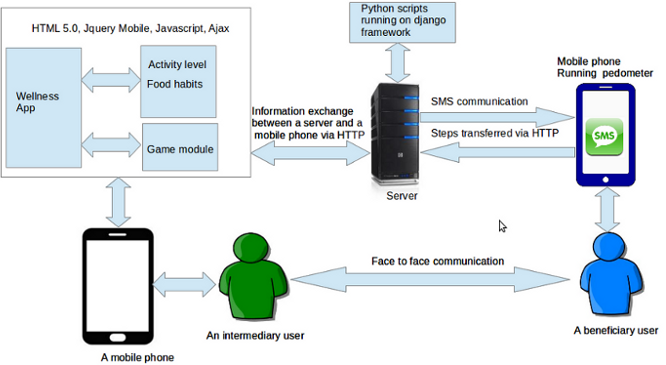
\epsfig{file=screen.png, height=1.8in, width=3.3in}
\caption{Information flow inside the system}
\label{figure:infflow}
\end{figure*}
\begin{figure}
\centering
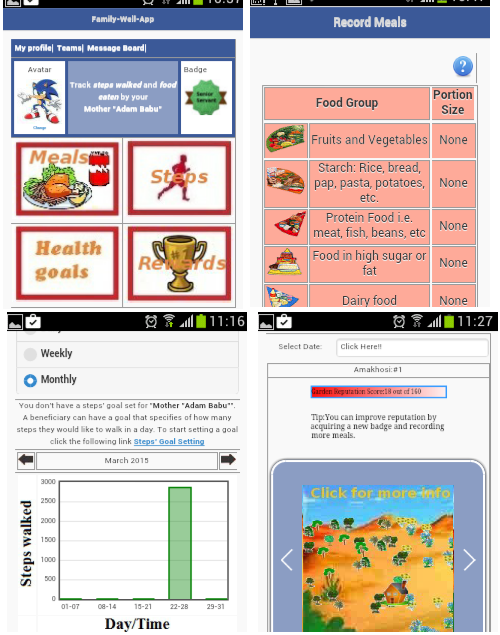
\epsfig{file=screens.png, height=3in, width=2.4in}
\caption{Sample screenshots from the system}
\label{figure:screens}
\end{figure}

\section{Methods}
\subsection{Contextual Inquiry}

We conducted a contextual inquiry using a series of semi-structured interviews
with 
a convenience sample of
diabetic patients at a diabetes and endocrinology clinic of Groote Schuur
Hospital in Cape Town. This was conducted in between March and May of the year
2013. The objective was to understand patterns in utilization of cellphone
technology among adults obese patients. This study was approved by the
respective institution's ethical review body.

We interviewed a total of thirty participants of which 67\% (20) were
females.  The average age of these participants was 53 years old with a
standard deviation of 11.8 years.  Almost 86\% (26) of participants were
above 40 years of age. A majority of the participants were either overweight or
obese and from low income suburbs of Cape Town. Nineteen participants were either
unemployed or on a disability grant. Participants were approached 
opportunistically as
they waited to see their physicians. To ensure confidentiality, interviews
were conducted in one of the vacant consultation rooms. One researcher and a
research assistant carried out the interviews. The main topics in these semi-
structured interviews were centred around participants' general utilization of
mobile phones, whether they seek help from intermediaries, and, if so, who their 
preferred intermediaries are.

Although eighteen participants had access to smartphones, utilization of
features was not beyond SMS and voice in majority of the participants. Out of
26 people whom were forty years of age and above, not more than eight had
already used Internet-based services (e.g. e-mail, WhatsApp, general Internet
browsing, Facebook). This suggests that majority of the aged
participants were likely to be less conversant with cellphone technology. Only
three participants had used their cellphones in management of their health,
to look for information on the Internet and to participate in social
support groups on Facebook. Only one participant had used a pedometer before.

We also
found that twenty participants had asked for informal help from
intermediaries before, in tasks such as: (1) to setup or configure services
and apps on their phones (e.g. Whatsapp, Facebook); (2) to be taught   how to
operate or navigate through certain features (e.g. a phone book of a new or
unfamiliar cellphone, Whatsapp); and (3) to be helped in interacting with
certain features such as SMS, Internet browsing etc. The level of dependence
on intermediaries varied depending on frequency of tasks at hand. Tasks such
as configuration of services and apps or teaching of individuals occur only at
the beginning when there is a new application or device. When participants
are not capable of interacting with applications that they use daily, then
they seek help more frequently. For either of these tasks, participants
chose trusted individuals to act as their intermediaries, typically
their children and grandchildren or, less frequently, children of relatives, family
friends, or someone at a cellphone shop. 23 out 30 participants preferred to have family
members act as their intermediaries.

Apart from utilization of help from intermediaries, we also observed that some
of the participants share their phones with their intermediaries. Children
borrow  their parents' phones to search for school materials on the Internet
or to use social network services such as Facebook or Mxit. For instance one
participant who had a Blackberry smartphone reported that she does not use
Internet on her phone but her kids use it to do their assignments. This is an
example of shared device use.

Our findings from this contextual enquiry indicate that  a majority of
the aged participants relied on expertise of their younger family members in
solving problems on both setting up of cellphones and interacting with
specific applications.  The majority of responses show that these
participants were assisted by their sons, daughters, and grandchildren. 
Based on this observation, we decided to implement a technology that can be
utilized through young intermediaries in a family. This finding 
motivated the use of gamification and the choice of intermediaries age
group in phases of evaluation that are explained in the next sub-sections.

\subsection{Iterative Design and Evaluation I}

We conducted two iterations of design. The first iteration started in July
2013. We developed the first prototype of a web application. This prototype
could allow users to self-monitor their diet and walking patterns. In
addition, we implemented a reward system that paired a beneficiary user with
an intermediary user in a team that could compete with other teams. Scores for
each team are presented as points, badges, and the appearance of fish and plants
in the 
tanks and botanical gardens. Within each botanical garden and fish tank, there
was a Facebook social plug-in that allowed users from different teams to
comment on or like each other. We also utilized Facebook groups to remind
users to engage with the application.

In order to test our application, we recruited participants through an NGO
based in Cape Town called ``\textbf{\textit{Mamelani Projects}}''. This NGO
carries out outreach programs on health education in less privileged
communities. Mamelani trains women them on
issues of HIV/AIDS, nutrition, and gender equality. 
The NGO agreed to help us to recruit participants
among people they were training. We gave them the following recruitment
criteria: (1) we want participants who were aged 35 or above and (2) those
participants must have an intermediary to help them. The NGO helped in
identifying the targeted participants in Philippi township, where the
NGO was conducting its own activities. T We recruited a total of
six participants whom were women above middle age (>=35 years of age).

After recruitment of the six adults, each one of them brought an intermediary
to work together with them in a pair. Three intermediaries were girls in
between 19-23 years of age. The remaining three intermediaries were boys aged
between 14 and 19 years of age. 
We informed participants about the objectives of the study,
that logs on their usage of the phones would be collected, and about 
their rights as research participants.
All participants (intermediaries and
beneficiaries) signed consent forms except for intermediaries who were minors.
These minors signed assent forms that were approved by their respective
parents/guardians. 
After signing of consent and
assent forms, intermediaries were trained on how to use the app. We deployed
the application to the field from the end of October 2014 to beginning of
December 2014. In order to control the application environment, and limit 
potential complications from deploying the intervention on multiple platforms, 
each pair of participants was given one Android phone (Samsung
GT-S5300) running the pedometer app. Participants were required to utilize the
web application hosted in our institution's server. We gave out  airtime as an
incentive to each participant including intermediaries. Every week each
participant got ZAR30 (\~US\$3) worth of airtime.

In that period of deployment, only two pairs of users engaged with the system
for more than a few days. Both of these two pairs consisted of a beneficiary 
and an  intermediary
living in the same house--- the pairs consisted of mothers working with their
sons. One of these two pairs was very motivated and enthusiastic about the
system. But after some time they also got bored because they were not getting
any competition from other teams and they had attained all the challenges
within a short period of time. In a third pair, a girl was working with her
mother but they were not living together so it was difficult for her to commit
to the application. Intermediaries from the remaining two pairs showed
little enthusiasm in the project. We hypothesized this to be due to lack of both
motivation to engage with gamification and a lack of a prior social relationship 
between
the two users within each pair. Findings from this informative evaluation led to
another iteration in the design. It also informed the manner in which we were
going to conduct future evaluations.

We started another iteration of design in January 2015 to address the
drawbacks encountered during testing of the first prototype. In this new
version we improved the gamification part to make it more challenging and we
also integrated SMS reminders. In the next sub section we discuss the
evaluation of the improved system.
 
\subsection{Evaluation II}
After fixing the bugs, we conducted another round of evaluation. We approached
another group of participants who resided in another side of Philippi. The
recruitment was facilitated by the same NGO in Evaluation I. Before the
commencement of the study, the NGO advised that we withdraw from that area as
participants addressed some concerns regarding safety issues. The area was not
safe, hence experimental phones would pose risks to both participants and the
researcher. In response, we terminated this study and sought participants in 
Langa, which as a smaller and more central township is safer than Philippi.

As an aside, this incident highlights some of the limits and dangers of doing 
smartphone-based interventions in low-income areas~\cite{Molapo2015}.  
However, we still believe that this study has relevance, even for residents of Philippi.  Intermediated usage is not limited to smartphone applications. For example, while SMS campaigns are not specifically designed for intermediated interactions, it is
not inconceivable that a family member would assist a target beneficiary
in an informal proximate interaction~\cite{sambasivan2010}.

In Langa, we worked with a research facilitator who is a resident of Langa. The research assistant helped with the recruitment process. This time we adjusted criteria for recruitment based on lessons learned during the first deployment in Philippi. The criteria for recruitment were (1)~adults aged 35 and above with (2)~school-going 
children living with them or living nearby.

Prior to deployment we provided participants with information about the study.
Participants were made aware that the study's cellphone will be collecting
their information related to steps and diet and transfer it to the
researcher's computer at University of Cape Town. Participants who were minors
signed assent forms approved by their guardians/parents who were also part of
the study. All other participants signed consent forms.   We recruited a total
of nine adults (3 men and 6 women). Each adult brought one kid to act as their
intermediary hence they formed a pair. There were 3 boys and 6 girls. All
adults were relatives of the kids except for one adult who was the tenant of
the grandmother of her intermediary. All intermediaries were school-going
children but one.  We administered a questionnaire at baseline to collect
demographic information such as age, number of cellphone applications utilized by each group of participants. Only seven beneficiary participants completed the
baseline survey. All nine of the kids completed the baseline survey. The mean age
for adults was 49.3 years old (SD=7.9 years) while the mean age for kids
was 14 years old (SD=4.3). We compared the average number of applications on a cellphone utilized by each set of users by using the student's t-test. Intermediary participants had significantly interacted with more applications (M=5.4; SD=1.7) before
compared to beneficiary participants with (M=3.4; SD=1.5) applications
(t(14)=2.430; p=0.029; 95\% CI=3.765 to 3.795 applications). 

We trained each kid on how to use the prototype. Each pair of participants was
given one android phone installed with a pedometer and a link to access the
web application. We left the application in the field for three weeks. We
provided airtime as incentives to participants. Each adult received ZAR40
worth of airtime four times in a period of three weeks. In addition,
each pair was given 300MB of data to use on the Android phone. After three
weeks we conducted interviews with three intermediary participants and the five
beneficiary participants who engaged with the application for more than once.
Interviews were conducted in English since all the respondents were
comfortable with English.

Out of nine pairs of users, eight attempted to engage with the application for
at least one day in a period of three weeks. The average number of usage days
for these eight participants was 4.88 days with a standard deviation of  3.4
days. Two pairs used the application for only one day. The most active pair
used it for 11 days in total. 
While there were many problems that contributed to non-use, the primary barrier
was that the data bundles allocated for the study (300MB per phone) were 
expended earlier than expected.
In addition to the prescribed study use, they also used the
data bundle for other apps such as Whatsapp and downloading of games. We 
elected not to prohibit this since it has been shown that allowing non-prescribed
use can motivate ongoing prescribed usage~\cite{Schwartz2013}.
Ferreira~\cite{ferrplay2015} also emphasizes that non-prescribed uses should not be
discouraged within the context of ICTD as they can be viewed as  capabilities
that foster participation and engagement in ICTD projects.

Our synthesis on data collected through interviews uncovered several themes
related to social dynamics on usage of a persuasive personal health
informatics through intermediaries. We discuss these findings on the next
section.

\section{Findings}

On reflection of findings from both evaluation I and II,  we uncovered some
useful insights on social dynamics that had an influence on utilization of a
BCCS in our context. Usage of the app occurred when intermediaries had access
to an experimental phone. Most beneficiaries went to work during the day and
hence they carried the phone with them, and  also intermediaries went to
school during the day. Figure \ref{figure:hourpattern} below shows the pattern
of the time of which there were users' activities on the app in evaluation II.
From the graph, the peaks are shown at 5AM, 5-6PM, and 8PM. These are times
when intermediaries and beneficiaries were together.

When a pair meets, one of them would instigate the request to engage with
information on the app. Initiation of the request to engage and success or
failure in fulfilment of a request were determined by social rapport within a
pair, motivational triggers as the result of the app's features, and social
interactions among beneficiary participants. The mentioned factors played a
part in influencing help-seeking by beneficiaries and help-giving by
intermediaries. We present in detail about these factors on the following sub-
sections. In addition, we also present perceived health benefits on
utilization of the application. All the names used in presentation of findings
are pseudonyms in order to ensure confidentiality of participants' identities.

 \begin{figure}
\centering
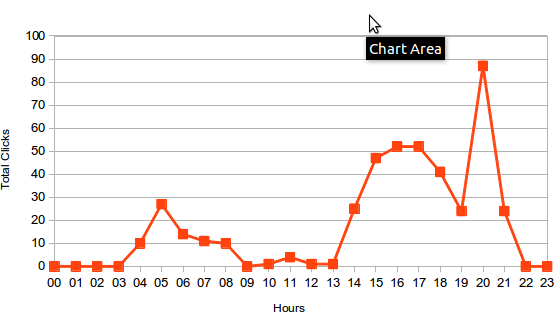
\epsfig{file=clicks_pattern_pilot2, height=2.5in, width=3.5in}
\caption{Total clicks on each hour of the day}
\label{figure:hourpattern}
\end{figure}
\subsection{Social Rapport}

We clustered each pair in evaluation II on its respective relationship type as
shown in Figure \ref{figure:relation}. In the parent-intermediary group, there
were four pairs. In the relative-intermediary group, there were three pairs,
and there was only one pair of where members didn't have a familial
relationship. We measured usage on each relationship type through three
dimensions and these are;the average number of days per participant; the
average number of sessions per participant; and the average number of clicks
per participant. We defined the beginning of a new session as when a user
activity is detected while there was no user activity for the past one hour.
If delay between activities is less than one hour it is then assumed that the
last session is still active. If a user comes back after one hour has elapsed
since the last detected user's activity then it is assumed they went away from
the app and now they are coming back for a new session.

Once members of a pair are together, interaction between them is initiated.
The success of this initiation depends on the nature of their social rapport
within a pair. In existing work on intermediaries within the context of ICTD,
human relationships play a pivotal role in encouraging or discouraging
engagement. In our context, we uncovered scenarios of how the relationship of
users within a pair played a significant role in facilitating or discouraging
requests for engagement. For members of a pair with a prior social
relationship, there was an indication of motivation for the two users to work
together. Within these pairs, intermediaries showed empathy and a sense of
ownership on interaction processes, and believed that the act of helping was
for a good cause as it had an instrumental value to the people they care
about. For instance \textbf{Lulama} (an intermediary from Langa), a 20 years
old girl, mentioned that the app was meaningful to her because she was helping
the person she cares about, and that was her mother. \textbf{Andile}, a 17
years old intermediary who was part of the study in Philippi, felt that it was
his duty to support his mother as she took care of him since the day he was
born. These are examples of how intermediaries were reciprocating the benefits
of a prior social relationship.

In a pair with no prior social relationship, negotiation for interaction may
not be successful even if one user within a pair is motivated to engage with
the system. For instance trust and social rapport hindered \textbf{Anele} (a
beneficiary user from Langa)(a 47 years old woman) from accessing the system.
She was working together with an intermediary that was not related to her as
we learned  during the interviews. The intermediary was the grand daughter of
her Landlord.

 \begin{figure}
\centering
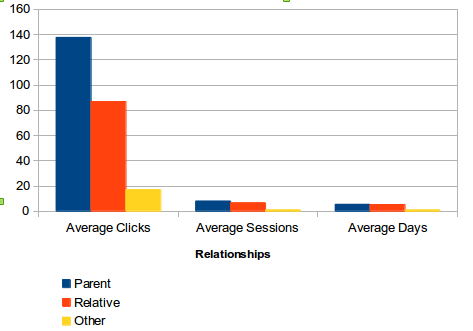
\epsfig{file=relationships, height=2.0in, width=3in}
\caption{Usage in three groups of relationships}
\label{figure:relation}
\end{figure}

When there was a prior social relationship (i.e. familial relationship), it
played part in mediating the success for negotiation of interaction. Either an
intermediary or beneficiary user would instigate a conversation that leads to
interaction with the wellness app and exchange of information between an
intermediary user and a beneficiary user. The phone was possessed by a
beneficiary user and if negotiation for interaction is successful, the phone
is passed from a beneficiary to an intermediary. If interaction was instigated
by an intermediary, an intermediary would request a beneficiary to provide
some information such as what food has been eaten by a beneficiary. Also an
intermediary might either view information inside the app for his or her own
consumption or share that information with a beneficiary user. If interaction
is instigated by a beneficiary user, most of the time they request
intermediaries to help them view certain information. In this scenario, there
were cases where intermediaries' autonomy was violated as beneficiaries
requested assistance at the time where intermediaries were either resting or
occupied by other activities. In these cases, a social relationship still had
to play a role in convincing intermediaries to fulfil requests from
beneficiaries.

Members of a pair with a prior social relationship demonstrated improved
relatedness within a pair compared to before. They mentioned that they were
conversing more often to talk about what is going on inside the app. The
conversation was fun in some of the participants when they made jokes about
what was happening inside the app.
\subsection{Motivation in Utilization of the app}
Motivational strategies that were implemented in the app and those that were
socially constructed as the result of engaging with information from the app,
played a vital role in persuading both beneficiary and intermediary users who
engaged with the application. These motivational strategies led to negotiation
of interaction. We discuss in detail these forms of motivational sources
below.
\subsubsection*{\textbf{Sources of Motivation in Beneficiaries}}

The most prominent motivational factor that drove beneficiaries to seek for
information derived from the app was steps comparison. Steps comparison was
socially constructed as majority of the beneficiaries lived not far from each
other.In cases where beneficiaries initiated the negotiation for interaction,
it was for the purpose of their health and secondly it was for comparisons
with other beneficiaries. This kind of comparison is referred as one form of
social comparison in the context of behavior change support 
system~~\cite{Oinas-kukkonen:psd}. This kind of comparison 
was not implemented in the app but it was instigated by the the existing social network. Some beneficiary users compared each other and this led to both social support, relatedness, and competition among beneficiary users. Beneficiary users who knew each other before organized themselves in informal support groups. Whenever beneficiary users met in these informal support groups, they talked about the steps walked or food they have been eating.
%\newline\newline

\userquote{\textbf{Nokhanyo} (beneficiary user), 57yrs, woman, from Langa}
{``I used to boss to others in the group like hahaha [She would giggle
 to the people she is interacting with] how many steps did you walk today 
 hahaha. I am getting there. I tell them I got some encouraging messages. 
 They would also say 'I got some too'. I tell them that I walked so many 
 kilometres today.''}
%newline
Through these informal discussions, beneficiary participants were encouraging
each other. There was also an indication of improved relatedness among
participants. People who were part of those informal support groups felt that
they were more related to each other compared to before using the app.

\userquote{\textbf{Nobantu} (beneficiary user), 50yrs, woman, from Langa} 
{``We [with other participants] didn't communicate so much before but 
now we communicate. Most of the time, we chat about this and we laugh.''}
``
\userquote{\textbf{Ndileka} (beneficiary user),  35yrs, woman, from Langa}
{``I am close to other people because of the steps. They would send 
you messages to ask `how many steps did you take?'. These are people that I 
didn't speak to here. Not to speak to, I mean others that I didn't have a 
really relationship with. I know them from here. It is just a hello, hello 
that's it. They send me messages `how many steps did you take today? Is this 
app working for you?'. There is this lady next door. She would come to me 
like ooh `how did that thing work for you and blah blah'. We were 
communicating more than before.''}

Competition with others was also partially linked to competition with self of
where beneficiaries challenged themselves by setting goals implicitly (without
writing them down). Goal setting pushed beneficiaries to do more in steps so
that they can beat others. For instance a person would ask her intermediary
about the number of steps they have walked in a particular day. Upon getting a
response from their intermediaries they would say that ``tomorrow I am going
to walk this number of steps''. But the main objective of setting these goals
is to have more steps than others. Goal setting is an important aspect in
health behavior change ~\cite{strecher1995goal}.

These findings suggest the role that activity and diet based social comparison
can play even in resource constrained environments. With typical behavior
change support systems from the west, this kind of comparison is always
provided through software functionality. In our system we implemented activity
and diet comparison through gamification design patterns such as points,
leader board, badges, botanical gardens, and fish tanks. Through these
features, each pair of users (a beneficiary and an intermediary) could be able
to make comparison with other teams. But our existing gamification features
appeared to be of less value to beneficiary users as they didn't really
understand the meaning of motivation strategies provided by gamification
although they interacted with those features through intermediaries. What they
valued most was their relationship with each other(beneficiaries) within the
context of the community they lived in.

\subsubsection*{\textbf{Motivational Sources in Intermediaries}} 

Each pair of users (an intermediary user and a beneficiary user) formed a team
that competed with other teams.  Some intermediaries pushed their beneficiary
users to walk more steps or to eat healthy due to two reasons. Firstly,
because they cared for the people they were helping. Secondly, because it gave
them more points to win the game against other teams.In cases where
intermediaries initiated the interaction, they did so to encourage
beneficiaries to do more so that their pair can win in gamification.
Gamification features in combination of a prior social rapport made some
intermediary users to perceive themselves as partial owners of the information
and value derived from the system. For instance one participant explained
actions that were carried out by the beneficiary she was helping as theirs.

\userquote{\textbf{Lulama}, an intermediary} {``When I saw the garden I was like yeah, our garden is looking beautiful. Lets do more. Lets take more steps. Lets eat more veges, because it is the veges and fruits that are important. One time she 
went to the clinic in town and she always walks to the clinic. It is up in 
town. That day I was motivated. She took more than four thousand steps. But 
mostly the garden . I like the garden. When I see the garden I say let's take 
more steps. Lets eat more veges.''}

Gamification features also led to competition among intermediaries. One
intermediary user explained how the badges played a role in challenging and
making him to compete with others. Badges were obtained in an incremental
process. Each badge had requirements that were specified by the minimum 
number of steps that needed to be walked by a beneficiary user, and the 
number of days a pair had used the system. Two intermediary participants mentioned how
the badges and competition motivated them to do more with their mothers 
The living metaphors such as botanical gardens and fish tanks triggered
social responses from some intermediary users. This phenomenon of computing
systems ability to present social cues to environment that trigger social
responses is discussed by Fogg ~\cite{foggpersuasivebook}. For instance we
asked one participant what was the size of fish in his tank and his response
was as follows, \textit{``They were medium sized because I wasn't really
feeding them.''} By feeding he meant recording of meals eaten by his
beneficiary user.
%\newline
Although beneficiaries were not so much concerned with gamification still intermediaries shared that information with them  as shown in the following excerpts. 

\userquote{\textbf{Lulama}, an intermediary} {``She saw the garden. The
first day she saw just the house and brownish [Desert]. She
is like `What is this'. I told her. She said `Aha! [Expressing
dissatisfaction]. It must look green and healthy'. And then
she saw the garden again and said `It is looking good.'
''}
\userquote{\textbf{Lwazi}, an intermediary} {``She doesn't understand the app. I just tell her that people are having ones twos threes and she laughs.''}
The above findings suggest that gamification resulted into a positive user 
experience on intermediaries and it had more value and meaning to them 
compared to beneficiary users. Most beneficiaries didn't understand the meaning of gamification functionality but upon proximate translation of output by intermediaries there were positive responses

\subsection{Perceived Benefits from our BCSS}

There were reported perceived benefits by beneficiary participants. For instance, the
process of recording meals led to cognitive dissonance in one participant.
Cognitive dissonance is where by an individual discovers that their beliefs
are not consistent to their actions. Oinas-Kukkonen et 
al~~\cite{Oinas-kukkonen:psd} discussed cognitive consistency as 
one of the key issues behind persuasive systems. People want their beliefs to be consistent with their actions. If there is an inconsistency, then it is likely  for them to become motivated to change their attitude or behavior in order to restore that consistency.  

\userquote{\textbf{Ndileka}, a beneficiary}
{``I think I like a bit everything about the app 
especially with food because I used to eat McDonalds. So I have to think of 
what I am going to eat first. I will think that I am eating big portions of 
carbohydrates and small portions of fruits. So now I have to balance, I 
have to eat fruits more than carbohydrates. With me it helps because now I 
can drink more water. I can eat more fruits than I used to.''}

Cognitive dissonance is achieved through self-monitoring as users see discrepancy between their beliefs and their actions. The purpose of self-monitoring is to trigger
individuals' consciousness to modifying their behaviour. This consciousness is fostered
through behaviour recording and observation. Self-monitoring is a very important aspect in cognitive behavior therapy. Health self-management programs usually ask participants to keep records of their activities, physiological variables and other health-related data; personal informatics systems can make this process simpler and easier. \cite{medynskiy2010salud}
Some participants became more aware of their eating and walking patterns. For instance one participant described that she would always try to avoid people's lifts on her way to the bus station so that she can walk more steps. If she stays at home for the whole day then she would make an effort to go to nearby shops just to buy airtime so that she can have some steps in her pedometer.

In other cases intermediary users explained how their beneficiary users were
controlling their eating habits as the result of interacting with information
derived from the app. For instance the meal chart from the app helped
\textbf{Nokhanyo} to reflect whether she was consuming meals that could
trigger the spike of her blood sugar level i.e carbohydrates.

%\newline\newline
\userquote{\textbf{Lulama}, an intermediary}{She [Nokhanyo] knows that `I am eating too 
much sugar. Let me lower my sugar by 500 calories in a week.' Yah it 
helps her that way. And she is diabetic. So when she tests herself she 
sees that she ate too much of something so she knows that she has to 
lower it. There is a chart. There is a plate. She looks at the plate and 
says that `I have eaten enough veggies but I need to eat more of this'. 
She doesn't eat meat that much.}

%\newline\newline
\userquote{\textbf{Lwazi}, an intermediary}
{It [The app] was really good because my 
mother was limiting herself on stuff like pies and fat food. I would tell 
her don't eat this don't eat that. She wasn't eating much vegetables but I 
was encouraging her to eat vegetables}

%\newline\newline

The application had a persuasive effect on beneficiary participants who
engaged with it, hence there is a feasibility for beneficiary user to derive
value from the information presented by a BCSS in our context. Without intermediaries some beneficiaries were not going to perceive the benefits of our BCSS as their consumption of information relied on intermediaries.  

\section{Discussion}

This work was developed based on existing literature of PHI and BCSS which is
dominated by research from the West. Our idea was to test if a PHI works by
laveraging existing intermediated technology use. As we found out during
contextual enquiry, intermediated technology use was common among aged
participants. So the approach attempted to utilize what already exists but
this time in the context of PHI.

Our findings uncover social dynamics that are important in understanding how
intermediated interactions can be leveraged to foster utilization of behavior
change support systems within family settings. The two important factors to
consider are (1) social rapport between an intermediary and a beneficiary as a
requirement for persuasion; and (2) differences in motivation strategies
between intermediaries and beneficiaries, we refer to this as parallel
persuasion.  We discuss these two factors in details below.

\subsubsection*{\textbf{Social Relationship on Engagement with a BCSS}}

The motivation strategies may work provided that an intermediary and a
beneficiary user have a prior social relationship. A prior social relationship
makes intermediaries to value the interaction as more meaningful. One of the
benefits of intermediaries valuing the interaction process as meaningful is
that; we can capitalize on intermediaries to play a role of persuaders for
health behavior change. We observed this phenomenon in pairs where an
intermediary and a beneficiary had a prior social relationship.

%\newline
%\newline
\userquote{\textbf{Nokhanyo}(a beneficiary user)}
 {Sometimes she (Lulama) 
used to shout at me. `No no you didn't eat that thing. Tell me what you 
ate in the morning. I saw you eating this. It seems there is nothing for 
fruits, peanuts. You must remind me to check you!'}
%\newline
%\newline
\userquote{\textbf{Lwazi}(an intermediary user), a 14 years old male from 
Langa}
{I would tell her don't eat this don't eat that. She wasn't 
eating much vegetables but I was encouraging her to eat vegetables.}
%\newline
%\newline

This is an example of how intermediaries with a prior social rapport can nudge
their beneficiaries to walk more steps or eat healthy. Intermediary users can
become a source of intent to persuade. In the work by Fogg
~\cite{fogg1998persuasive} mentioned in ~\cite{Oinas-kukkonen:psd}, intentions
to persuade can come from three sources and these are; from the people who
create or produce interactive technology; from people who give access to or
distribute the interactive technology to others for which in our case could be
intermediary users; and the people themselves who use or adopt an interactive
technology. The approach of using people supported by technology to persuade
other people is not new in the context of ICTD work. As we have seen in a
study in India that equipped health care workers with mobile phones of which
they could access persuasive messages and use them to persuade women on
maternal health issues~\cite{ramachandran2010mobile,ramachandran2010research}.
Our approach is more innate as intermediaries and beneficiaries meet in
natural settings and it can be more feasible of where persuasion is an ongoing
process. Therefore, prior social rapport is one the prerequisites in laveraging intermediaries in utilization of a BCSS.


\subsubsection*{\textbf{Parallel Persuasion}} 
Prior social rapport it self may not be sufficient for sustainability of engagement. Motivation strategies are needed in conjunction with a prior social rapport. Affective persuasion strategies are important in sustainability of engagement with a BCSS.  Unlike existing persuasion problems of where we design for one user; persuasion in our context is more complex as it involves both intermediary and beneficiary users. Despite of existing relationships between intermediary and
beneficiary users, intermediaries, may not always be willing to help regularly
and this might discourage beneficiaries and hence discontinue usage of a BCSS.
Kiesler et al.~\cite{kiesler:twi} found out that some parents became hesitant
to seek informal help from their children after they had encountered negative
experiences. We encountered this phenomenon during both contextual enquiry,
and preliminary interviews before evaluation II. Some of our participants
shared these negative experiences. For instance one participant mentioned that
sometimes it is difficult to seek help on using cellphone because their kids
are sometimes annoyed when they are constantly asked to help especially if it
the same task from last time. Therefore, it is important to minimize negative
experiences of beneficiaries by increasing engagement of intermediaries.

We have the task of persuading intermediaries to share information with
beneficiaries, and we also have the task of persuading beneficiaries to change
their health behaviors. From our findings, we see how persuasion strategies
between intermediaries and beneficiaries differ. For a beneficiary, the weight is more on perceived value of the information on health benefits and informal social comparison with other beneficiaries from the same community. Intermediaries put value on
game design elements and social comparison is within the context of
gamification. This suggests that persuasive strategies between intermediaries and beneficiaries differ. In our context, intermediaries were young and most of them had experiences in games. A previous study on application of gamification on product advertising\cite{v2014motivational} found out that a prior gaming experience predicts higher purchasing intentions. However there is a caveat in utilization of gamification among young people. A study by Koivisto and Hamari\cite{koivisto2014demographic} found that the usage of  a gamified system is highly affected by the novelty effect and this is more apparent on younger users compared to the old ones. As time passes by younger users tend to get bored with a gamified service. Also ease of use of gamification tends to decline with age \cite{koivisto2014demographic} with young users reporting systems to be easier use compared to their older counterparts.  


In addition, we have seen from above that intermediaries can introduce an intent to persuade apart from these informal social comparisons. The persuasion strategy to be used by each set of user can be examined during analysis of persuasion context as suggested in PSD \cite{Oinas-Kukkonen:foundation}  and BCSS \cite{Oinas-kukkonen:psd} models. This will determine of whether the persuasive functionality is for intermediaries layer or is for beneficiaries' layer.To engage beneficiaries we  can support direct activity and diet comparison among beneficiaries through the app but implementation of this needs to address issues of privacy. An application can be configured with privacy settings to allow aggregated information of beneficiaries to be kept private or shared with other teams. The aggregated information that is shared by different intermediaries can be clustered in a bar chart to facilitate social comparison. With gamification strategies on intermediaries, and direct comparison by intermediaries we can have persuasion strategies to cater for the two sets of users.

\section{Conclusions}

We have explored the extent to which we can leverage on intermediaries within
family settings to support utilization of behavior change support
systems(BCSSs) for health. We presented the social dynamics that one needs to
consider when designing a BCSS for health in the context of intermediated
interactions. We also discussed how persuasive functionality might work
considering the fact that we have two layers of persuasion. Our findings
suggest that it is feasible to take advantage of intermediated interactions to
support utilization of ICTs in health behavior change interventions.
   
This study has limitations in generalizations as we generated our insights
based on fewer iterations of evaluations. A larger ethnography study is needed
in understanding the contextual dynamics of an intermediated BCSS in detail.
Secondly, it is not known to what extent gamification mediated the intrinsic
motivation of both intermediaries and beneficiaries. In our current work we
are carrying out a control study to evaluate the extent to which gamification
has an impact on intrinsic motivation of both intermediaries and
beneficiaries. We seek to understand if intermediaries' intrinsic motivation
to assist in self-monitoring can be enhanced by gamification as well as an
intrinsic motivation of beneficiaries in engaging in self-monitoring of
health. We are comparing two systems; one with gamification; and another one
without gamification.

%\end{document}  % This is where a 'short' article might terminate

%ACKNOWLEDGMENTS are optional 

\section{Acknowledgments} 

This work would have
not been possible without the generous funding of Centre of Excellence(CoE)
and HPI Research School at University of Cape Town.

%
% The following two commands are all you need in the
% initial runs of your .tex file to
% produce the bibliography for the citations in your paper.
%small{
\bibliographystyle{abbrv}
\bibliography{sigproc} %} % sigproc.bib is the name of the Bibliography in this case
% You must have a proper ".bib" file
%  and remember to run:
% latex bibtex latex latex
% to resolve all references
%
% ACM needs 'a single self-contained file'!
%
%APPENDICES are optional
%\balancecolumns


\end{document}
